
\paragraph{Diffusione del campo magnetico in un cilindro conduttore indefinito}
Si considera il conduttore in sezione nel piano $x,y$, rappresentato come una circonferenza di raggio $a$
in cui circola una corrente $\vec{J}$ tale che
$$
\vec{J}(p',t) = J_z(r,t)\vec{e}_z
$$
\begin{figure}[H]
\centering
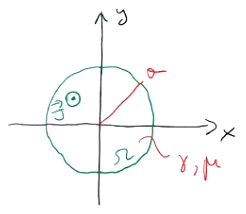
\includegraphics[width = 0.3\linewidth]{conduttore_cilindrico_indefinito}
\end{figure}

$$
\begin{aligned}
&\nabla\times\vec{E} = -\frac{\partial\vec{B}}{\partial t} \\
&\nabla\times\vec{H} = \vec{J}
\end{aligned}\quad \in\ \Omega \quad
\begin{aligned}
&\nabla\cdot\vec{J}=0\ \text{MQS}\\
&\vec{J} = \gamma\vec{E}
\end{aligned}
$$
Supponendo che il materiale sia lineare si possono sostituire i campi $\vec{E}$ e $\vec{B}$ usando le costanti
$\gamma$ e $\mu$
$$
\nabla\times\frac{\vec{J}}{\gamma} = -\frac{\partial}{\partial t} \left(\mu\vec{H}\right)
$$
applicando nuovamente il rotore e ricordando il teorema di Schwarz
$$
\frac{1}{\gamma}\nabla\times\nabla\times\vec{J} = -\frac{\partial}{\partial t} \left(\mu\nabla\times\vec{H}\right)
= - \frac{\partial}{\partial t} \left(\mu\vec{J}\right)
$$
ricordando la solenoidalità di $\vec{J}$
$$
\frac{1}{\mu\gamma} \left[\cancel{\nabla\left(\nabla\cdot\vec{J}\right)} - \nabla^2\vec{J}\right] = -\frac{\partial}{\partial t} \vec{J}
$$
in conclusione
$$
\frac{\partial \vec{J}}{\partial t} = \frac{1}{\mu\gamma}\nabla^2\vec{J}
$$
L'equazione è formalmente simile a quella vista per la diffusione del campo magnetico, cambiano le condizioni
al contorno.

In questo caso la $\vec{J}$ ha solo componente $z$ e in coordinate cilindriche il laplaciano diventa
$$
\nabla^2J_z = \nabla\cdot\nabla J_z = \frac{1}{r}\frac{\partial}{\partial r} \left(r \frac{\partial J_z}{\partial r}\right)
$$
quindi l'equazione di diffusione diventa
$$
\frac{\partial J_z}{\partial t} = \frac{1}{\mu\gamma} \frac{1}{r} \frac{\partial}{\partial r}\left(r \frac{\partial J_z}{\partial r}\right)
$$

Si usa ancora una volta il metodo dei fasori supponendo che la corrente abbia un andamento sinusoidale
$$
J_z(r,t) = \Re\left\{\overline{J}_z(r)e^{j\omega t} \right\}
$$
derivando si ottiene una delle \href{https://it.wikipedia.org/wiki/Equazioni_di_Bessel}{Equazioni di Bessel} la cui 
soluzione si ottiene in termini delle funzioni speciali di Bessel
$$
j\omega\mu\gamma \overline{J}_z(r) = \frac{1}{r} \frac{\partial}{\partial r} \left(r\frac{\partial}{\partial r} \overline{J}_z\right)
$$
si riporta la forma canonica indicando con $k^2 = j\omega\mu\gamma$
$$
\frac{\partial}{\partial r} \left(r\frac{\partial}{\partial r}\overline{J}_z\right) - k^2r\overline{J}_z = 0
$$
si evidenzia con $k^2$ lo stesso termine precedentemente evidenziato per la diffusione del campo magnetico,
analogamente quindi si riportano le condizioni limite per la diffusione.

%\begin{itemize}
%\item 
$a\gg\delta(\omega)$ si ritiene ragionevolmente che la densità di corrente $\vec{J}$ sia distribuita 
lungo le pareti del cilindro, in una corona circolare, approssimativamente nel seguente modo
\begin{figure}[H]
\centering
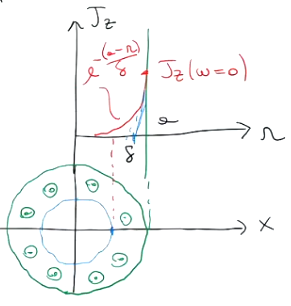
\includegraphics[width = 0.3\linewidth]{cilindro_indefinito}
\end{figure}
la sezione centrale non contiene corrente. La sezione utile è $\pi\left(a^2-b^2\right)$ con $b\simeq a- \delta(\omega)$ quindi anche la resistenza del conduttore dipenderà dalla frequenza
$$
\frac{R(\omega)}{L} = \frac{\eta}{S(\omega)} = \frac{\eta}{\pi\left(a^2 - (a-\delta)^2\right)} = \frac{\eta}{\pi\left(2a\delta - \cancel{\delta^2}\right)} \simeq \frac{\eta}{\pi 2 a \delta(\omega)} = \frac{\eta\sqrt{\mu\omega\gamma}}{\pi 2 a \sqrt{2}}
$$
a meno di termini correttivi del coefficiente, la dipendenza della resistenza dalla pulsazione è $R(\omega)\propto \sqrt{\omega} $
Analogamente alla laminazione per abbattere le perdite, è previsto l'intreccio di più conduttori isolati tra loro
per ridurre le perdite dovute all'effetto pelle ed aumentare la superficie utile di conduzione a parità di volume di 
materiale utilizzato.
%\end{itemize}
Vengono utilizzati cavi \href{https://it.wikipedia.org/wiki/Filo_litz}{LITZ} per applicazioni particolari in alta 
frequenza costruiti secondo questa metodologia.

Si confronta un cavo di raggio $a$ con un equivalente LITZ formato da $n$ conduttori di raggio $b$,
imponendo $nb^2 = S_0$ allora $R_n < R_1$ se $nb^2 > 2a\delta(\omega)$ si determinano infine $n$ e $b$.

Ad esempio per un conduttore in rame a \SI{100}{\kilo\hertz}, con permeabilità prossima a quella del vuoto
$\mu = \mu_0 $ e conducibilità $\gamma= \SI{5.8e7}{\siemens\per\meter}$ lo spessore di penetrazione è
$$
\delta_{Cu} = \sqrt{\frac{2}{\gamma\mu\omega}} \simeq \SI{0.21}{\milli\meter}
$$
Con una sezione $S_0(\omega = 0)$ pari ad \SI{1}{\milli\meter^2} si ha una resistenza per unità di lunghezza
$$
\frac{R_1}{L} = \frac{\eta}{S_1} = \frac{\SI{0.17e-7}{}}{\pi\delta_{Cu} 2\sqrt{\frac{S_0}{\pi}}} = \SI{0.023}{\ohm\per\meter}
$$
se si suppone invece la resistenza usando un solo spessore di penetrazione, si vogliono calcolare i conduttori
necessari
$$
\frac{R_n}{L} = \frac{\eta}{\pi n\delta^2}
$$
$$
\frac{S_1}{\pi\delta_{Cu}^2} = n = 5.4
$$
analizzando ovviamente il giusto trade-off tra il costo del cavo e le perdite accettabili. Solitamente le linee 
elettriche in alta tensione sono costituite da conduttori con anima interna in acciaio, dalle buone proprietà
meccaniche ma peggiori proprietà elettriche e ricoperti esternamente da conduttori in alluminio i quali sono
effettivamente interessati al passaggio della corrente.

\subparagraph{Correnti parassite in un cilindro conduttore completamente penetrato dal campo B} $\vec{B} = B_z(t)\vec{e}_z$ con $B_z(t) = B_m\cos\left(\omega t\right)$
In questa condizione $\delta(\omega)\gg a$, la corrente è dunque uniforme, si applica la legge di Faraday-Neumann
ad una linea $\Gamma$ chiusa interna alla sezione del conduttore.
\begin{figure}[H]
\centering
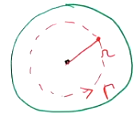
\includegraphics[width = 0.25\linewidth]{circuitazione_conduttore_massiccio_cilindrico}
\end{figure}
$$
\oint_\Gamma \vec{E}\cdot\hat{t}dl = - \frac{d}{dt}\Phi_\Gamma \Rightarrow 2\cancel{\pi} \cancel{r} E_\varphi = \cancel{\pi} r^{\cancel{2}} \omega B_m\sin\left(\omega t\right)
$$
$$
E_\varphi = \frac{\omega B_m}{2}\sin\left(\omega t\right)r
$$
La potenza assorbita per effetto Joule a causa delle correnti parassite
$$\begin{aligned}
p^{(a)} &= \iiint_\Omega \gamma E^2 dV = L\int_0^{2\pi}d\varphi r \int_0^a\gamma E^2_\varphi dr = L2\pi \int_0^a \gamma \left(\frac{\omega B_m}{2}\sin\left(\omega t\right)r\right)^2rdr =\\
&= 2\pi L \gamma \left(\frac{\omega B_m}{2}\sin\left(\omega t\right)\right)^2\frac{a^4}{4} 
\end{aligned}
$$
La potenza media sul periodo $T = \frac{2\pi}{\omega}$ ancora una volta è
$$
<p^{(a)}>_T = \frac{1}{T} \int_0^T p^{(a)}(t')dt' = 2\pi L\gamma \frac{\omega^2B_m^2}{4\cdot 2} a^2 \cdot \frac{a^2}{4}
$$
per unità di volume ricordando che il volume del cilindro è $V = \pi a^2 L $
$$
\frac{<p^{(a)}>_T }{V} = \frac{1}{2}\gamma\frac{\omega^2B_m^2a^2}{8}
$$
Anche in questo caso dipende dal quadrato della frequenza e di una grandezza caratteristica del materiale.
\newpage
\subsection{Bilanci di energia per un sistema elettromagnetico}
Si consideri un circuito RLC
\begin{figure}[H]
\centering
\begin{circuitikz}
\draw (0,2) to [R,i>^=$i(t)$,l_=$R$] (2,2) to [L,l_=$L$] (4,2) to [C,v^=$v_c(t)$,l_=$C$] (4,0) to (0,0);
\draw (0,2) to [open,v=$v(t)$] (0,0);
\end{circuitikz}
\end{figure}
La potenza assorbita dal circuito nell'istante $t$
$$
P^{(a)}_{RLC}(t) = v(t)i(t) = Ri^2 + \frac{d}{dt}\left(\frac{1}{2}Li^2 + \frac{1}{2}Cv_C^2\right)
$$
complessivamente
$$
-P_{\text{out}} = P_\text{in} = P_\text{diss} + \frac{d}{dt} W
$$
Lo stesso bilancio può essere scritto per una teoria di campo, considerata la normale uscente dalla
superficie di controllo
$$
P_\text{in} = -\iint_{\partial\Omega} \vec{S}\cdot\hat{n}dS = \iiint_\Omega P_\text{diss}(p')dV + \frac{d}{dt}\iiint_\Omega w(p')dV
$$
dove $\vec{S}$ è il flusso di potenza uscente per unità di superficie, $P_\text{diss}$ è la densità di potenza 
dissipata per unità di volume, e $w$ è la densità di energia interna per unità di volume.
Questa tipologia di bilancio vale per qualsiasi sistema.

In forma locale
$$
-\iiint_\Omega \nabla\cdot\vec{S}dV = \iiint_\Omega P_\text{diss}dV + \frac{d}{dt} \iiint_\Omega wdV
$$
Preso un volumetto di controllo $\Delta\Omega$ al quale si applica questo bilancio e si esegue il limite
$\text{Vol}(\Delta\Omega)\to 0 $ intorno a $p'$
$$
-\nabla\cdot\vec{S} = P_\text{diss} + \frac{\partial w}{\partial t}
$$
$$
[S] = \si{\watt\per\meter^2}\quad [P_\text{diss}] = \si{\watt\per\meter^3}\quad [w] = \si{\joule\per\meter^3}
$$
\newpage
\paragraph{Bilancio energia in Elettromagnetismo}
Si suppone che il volume $\Omega$ sia sede di campi elettromagnetici retti dalle equazioni di Maxwell complete
$$
\nabla\cdot\vec{B} = 0\quad \nabla\cdot\vec{D} = \rho_\text{lib}\quad \nabla\times\vec{E} = -\frac{\partial\vec{B}}{\partial t}\quad \nabla\times\vec{H} = \vec{J}_\text{lib} + \frac{\partial\vec{D}}{\partial t}
$$
$$
\vec{B} = \mu_0\left(\vec{H}+\vec{M}\right)\quad \vec{D} = \varepsilon_0\vec{E} + \vec{P}
$$
Si moltiplica la terza per $\vec{H}$ e la quarta per $\vec{E}$
$$
\vec{H}\cdot\nabla\times\vec{E} = -\vec{H}\cdot\frac{\partial\vec{B}}{\partial t} \qquad \vec{E}\cdot\nabla\times\vec{H} = \vec{E}\cdot\vec{J}_\text{lib} + \vec{E}\cdot\frac{\partial\vec{D}}{\partial t}
$$
Si sottrae la prima alla seconda
$$
\vec{E}\cdot\nabla\times\vec{H} - \vec{H}\cdot\nabla\times\vec{E} = -\nabla\cdot\left(\vec{E}\times\vec{H}\right)=
\vec{E}\cdot\vec{J}_\text{lib} + \vec{E}\cdot\frac{\partial\vec{D}}{\partial t} + \vec{H}\cdot\frac{\partial\vec{B}}{\partial t}
$$
Rinominando $\vec{E}\times\vec{H} = \vec{S}$ chiamato \href{https://it.wikipedia.org/wiki/Teorema_di_Poynting}{vettore di Poynting} si ottiene proprio il bilancio di energia
in forma locale precedentemente ricavato. Sostituendo le definizioni di $\vec{B}$ e $\vec{D}$ si ottiene
$$
-\nabla\cdot\vec{S} = \vec{E}\cdot\vec{J}_\text{lib} + \frac{\partial}{\partial t}\left(\frac{1}{2}\varepsilon_0E^2 + \frac{1}{2}\mu_0H^2\right) + \vec{E}\cdot\frac{\partial\vec{P}}{\partial t} + \vec{H}\cdot\frac{\partial}{\partial t} \left(\mu_0 \vec{M}\right)
$$
In forma integrale
$$\begin{aligned}
-\iint_{\partial\Omega}\vec{S}\cdot\hat{n}dS &= \iiint_\Omega\vec{E}\cdot \vec{J}_\text{lib}dV + \frac{d}{dt}\iiint_\Omega \frac{1}{2}\varepsilon_0E^2dV + \frac{d}{dt}\iiint_\Omega \frac{1}{2}\mu_0H^2dV +\\ 
&+ \iiint_\Omega\vec{E}\cdot\frac{\partial \vec{P}}{\partial t} + \vec{H}\cdot\left(\mu_0\frac{\partial\vec{M}}{\partial t}\right)dV
\end{aligned}
$$
Se le sorgenti sono tutte prossime all'origine e si considera una sfera $\Omega$ di raggio $r\to\infty$ i campi
sono tutti normali all'infinito, in particolare $\vec{E}$ va come $1/r^2$ e $\vec{H}$ va come
$1/r^3$ quindi il prodotto $\vec{E}\times\vec{H}$ va come $1/r^5$ moltiplicato per una superficie
diventa $1/r^3$. L'energia elettromagnetica è dunque concentrata attorno le sorgenti se i campi sono
quasi-stazionari.

L'unico modo di avere potenza irradiata a grande distanza è avere $\vec{E}$ e $\vec{H}$ che scalino come $1/r$,
il vettore di Poynting andrà come $1/r^2$, ottenendo una potenza irradiata costante sulla superficie, ciò
avviene con la propagazione elettromagnetica, in condizioni non stazionarie.

\newpage
\paragraph{Sistemi conservativi} $P_\text{diss} = 0$ la potenza in ingresso sarà concentrata in variazione di
energia interna.
A seconda della tipologia di sistema e della variazione più importante di energia si ha la condizione 
\begin{itemize}
\item EQS $\frac{\partial \vec{B}}{\partial t}$ trascurabile
\item MQS $\frac{\partial \vec{D}}{\partial t}$ trascurabile
\item Condizioni stazionarie $\frac{\partial \vec{B}}{\partial t},\ \frac{\partial \vec{D}}{\partial t}$ trascurabili
\end{itemize}
Nel terzo caso, preso un bipolo generico associato ad una corrente $i$ ed una tensione $v$, il flusso
del vettore di Poynting
$$
-\iint_{\partial\Omega} \vec{S}\cdot\hat{n}dS = v\cdot i = P_\text{in}
$$
%1:24:42
